\documentclass[a4paper]{article} 
\usepackage{graphicx} 
\usepackage[ngerman]{babel} 
\usepackage[ansinew]{inputenc} 
\usepackage[T1]{fontenc} 
\usepackage{tgpagella} 
\usepackage{geometry} 
\usepackage{color} 
\usepackage{microtype} 
\usepackage{minted}
\usepackage{caption}
\usepackage[headsepline,footsepline]{scrpage2}
\usepackage{textcomp}
\usepackage{pdfpages}
\usepackage{mdframed}



\makeatletter
\renewcommand\minted@pygmentize[2][\jobname.pyg]{
  \def\minted@cmd{pygmentize -l #2 -f latex -F tokenmerge
    \minted@opt{gobble} \minted@opt{texcl} \minted@opt{mathescape}
    \minted@opt{startinline} \minted@opt{funcnamehighlighting}
    \minted@opt{linenos} -P "verboptions=\minted@opt{extra}"
    -O encoding=UTF-8,outencoding=iso-8859-1 -o \jobname.out.pyg #1}
  \immediate\write18{\minted@cmd}
  % For debugging, uncomment:
  %\immediate\typeout{\minted@cmd}
  \ifthenelse{\equal{\minted@opt@bgcolor}{}}
   {}
   {\begin{minted@colorbg}{\minted@opt@bgcolor}}
  \input{\jobname.out.pyg}
  \ifthenelse{\equal{\minted@opt@bgcolor}{}}
   {}
   {\end{minted@colorbg}}
  \DeleteFile{\jobname.out.pyg}}
\makeatother


\title{Dokumentation - 6 Übung}
\author{Roman Lumetsberger}
\date{\today}

\newmintedfile[ccode]{cpp}{
               linenos,
               numbersep=5pt,
               frame=lines,
               framesep=2mm
}

\newmintedfile[javacode]{java}{
               linenos,
               numbersep=5pt,
               frame=lines,
               tabsize=2,
               framesep=2mm,
}
\newmintedfile[csscode]{css}{
               linenos,
               numbersep=5pt,
               frame=lines,
               tabsize=2,
               framesep=2mm,
}
\newmintedfile[sqlcode]{sql}{
               linenos,
               numbersep=5pt,
               frame=lines,
               tabsize=2,
               framesep=2mm,
}
\captionsetup{
  font=footnotesize,
  justification=raggedright,
  singlelinecheck=false
}


\newcommand{\srcDir}{../Beispiel/src/at/lumetsnet/caas/}
\newcommand{\testDir}{../Beispiel/test/at/lumetsnet/caas/test/}

\definecolor{lineColor}{RGB}{151,0,0}
\pagestyle{scrheadings}
\clearscrheadfoot
\begin{document}
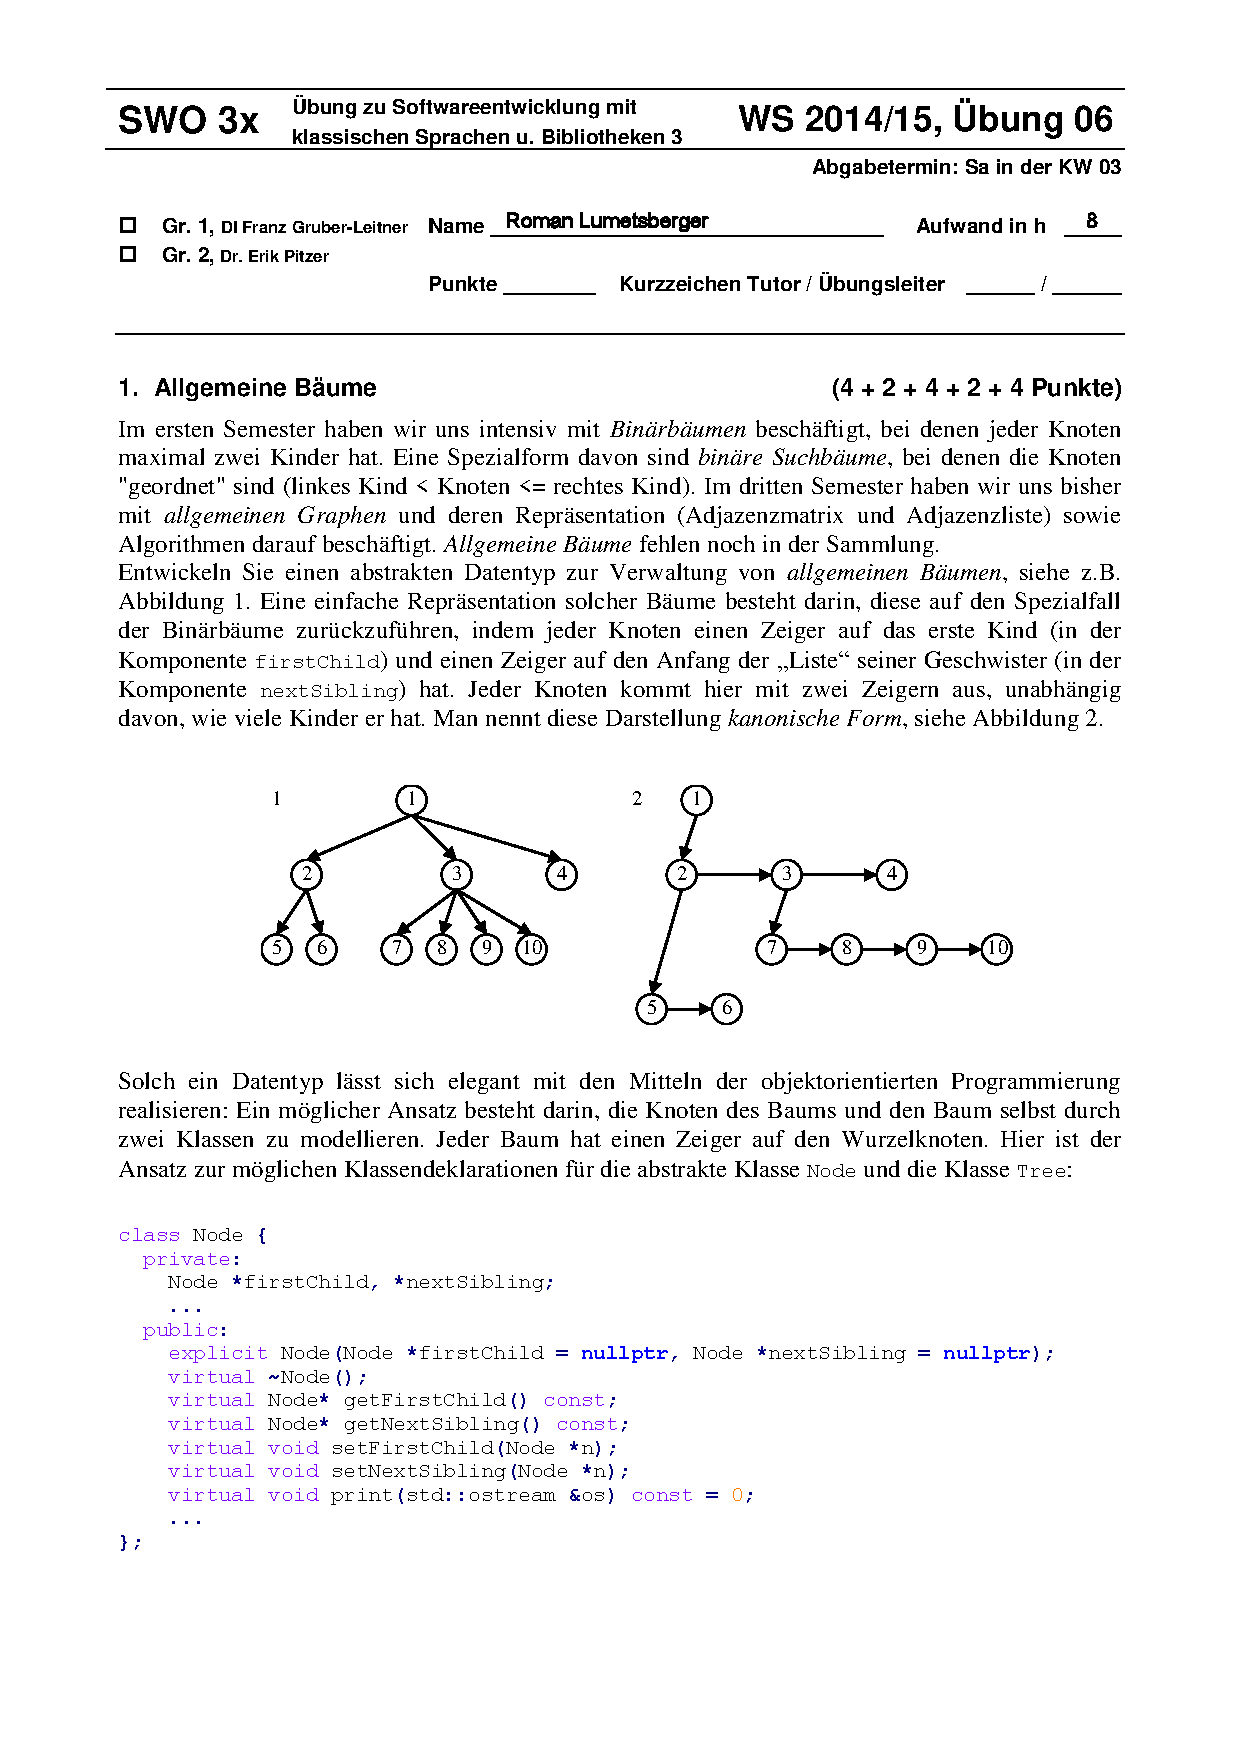
\includepdf[pages=-]{angabe.pdf}

\ihead{SWO3 WS 2014/15 - �bung 06}
\ifoot{Roman Lumetsberger}
\cfoot{1310307026}
\ofoot{Seite \pagemark}

\section{Aufgabe 1 - Allgemeine B�ume }
\subsection{Anmerkungen}
Diese Aufgabe wird mit der \textit{minilib} umgesetzt und dadurch werden alle Methoden mit einem gro�en Anfangsbuchstaben benannt, da dies in der minilib Konvention ist.

\subsection{L�sungsidee}
Der Baum wird, wie in der Angabe vorgegeben, mit den 2 Klassen \textit{Node} und \textit{Tree} umgesetzt.

\subsubsection{Node}
Diese Klasse implementiert einen Knoten im Baum. Dabei hat ein solcher Node genau einen Zeiger auf einen Kindknoten und einen Zeiger auf den n�chsten Geschwisterknoten. Mit diesen beiden Zeigern k�nnen allgemeine B�ume umgesetzt werden. \newline

\begin{itemize}
\item Die Zugriffe auf die Datenkomponenten werden mit Zugriffsmethoden gew�hrleistet.  
\item Der \textit{Destruktor} l�scht sowohl den Kind- als auch den Geschwisterknoten und gibt den Speicher frei. 
\item Die Methode \textit{Clone} kopiert sowohl den Geschwister- als auch den Kindknoten. Diese Methode wird verwendet um eine Kopie des Baumes anzulegen.
\end{itemize}

\subsubsection{Tree}
Die Klasse \textit{Tree} implementiert die geforderten Methoden um einen allgemeinen Baum mit Hilfe der Klasse \textit{Node} aufzubauen.

\begin{itemize}
\item \textit{InsertChild} f�gt einen Kindknoten unter den gegebenen Knoten ein. Sollte der \textit{Parent} gleich nullptr sein, dann wird dieser Knoten als Root-Knoten verwendet. Dabei ist zu beachten, dass der \textit{Parent} auch wirklich Teil des Baumes ist.
\item \textit{DeleteSubtree} l�scht einen Teilbaum und gibt auch seinen Speicher frei.
\item  \textit{Clear} setzt nur den Root-Knoten auf nullptr und \textbf{gibt keinen Speicher frei}.
\item \textit{GetSize} berechnet die akuelle Anzahl an Knoten im Baum.
\end{itemize} 
\textbf{Kopierkonstruktor}  \newline
Der Kopierkonstruktor kopiert den gesamten Baum, indem er die Clone Methode des Root-Elements verwendet und dadurch auch alle Kinder und Geschwister kopiert werden.\newline
\textbf{Zuweisungsoperator}  \newline
Auch dieser Operator kopiert den gesamten Baum, indem er alle Nodes kopiert. Hier ist zu beachten, dass der alte Baum freigegeben werden muss. Dabei werden alle Nodes freigegeben und k�nnen danach nicht mehr verwendet werden.

\section{Aufgabe 2 - Hierarchisches Dateisystem }
\subsection{Anmerkungen}
Auch diese Aufgabe wird mit der \textit{minilib} umgesetzt und dadurch werden alle Methoden mit einem gro�en Anfangsbuchstaben benannt, da dies in der minilib Konvention ist.

\subsection{L�sungsidee}

\subsubsection{Node Klassen}
Die ben�tigten Klassen werden, wie in der Angabe vorgegeben, abgeleitet und die Methoden entsprechend implementiert. Die Einschr�nkung der Klasse \textit{File}, keine Kinder zu haben, kann durch das �berschreiben der Methode SetFirstChild sichergestellt werden. \newline

\subsubsection{Filesystem}
Diese Klasse implementiert die geforderten Methoden. Dabei wird diese Klasse von \textit{Tree} abgeleitet. \newline
Zu den in der Basisklasse implementierten Methoden wird eine weitere ben�tigt, die es erlaubt einen Node im Tree anhand eines gegebenen Pfades zu finden. Diese muss also ausgehend vom Root alle Geschwister durchsuchen und bei jeden Seperator eine Ebene tiefer weitersuchen. \newline
Hier wird die Funktion \textit{strtok} der C-Standardbibliothek verwendet.

\begin{itemize}
\item \textbf{Touch}: F�gt einen neuen Knoten der Klasse \textit{File} in den Baum ein. 
\item \textbf{Mkdir}: F�gt einen neuen Knoten der Klasse \textit{Directory} in den Baum ein.
\item \textbf{Rm}: Sucht und l�scht den Knoten. Dabei muss beachtet werden, dass der gefundene Knoten vom Typ \textit{File} ist.
\item \textbf{Rmdir}: Verwendet \textit{DeleteSubtree}, um das Verzeichnis zu l�schen. Dabei muss gepr�ft werden, dass es keine Kindknoten gibt(also das Verzeichnis leer ist).
\item \textbf{Ls}: Verwendet \textit{Print}, um das Dateisystem auszugeben.
\end{itemize}

\pagebreak
\subsection{Sourcecode}
\textbf{Node.h}
\ccode{../Beispiel/Tree/include/Node.h}
\textbf{IntNode.h}
\ccode{../Beispiel/Tree/include/IntNode.h}
\textbf{Tree.h}
\ccode{../Beispiel/Tree/include/Tree.h}
\textbf{FSNode.h}
\ccode{../Beispiel/Tree/include/FSNode.h}
\textbf{Directory.h}
\ccode{../Beispiel/Tree/include/Directory.h}
\textbf{File.h}
\ccode{../Beispiel/Tree/include/File.h}
\textbf{FileSystem.h}
\ccode{../Beispiel/Tree/include/FileSystem.h}

\textbf{Node.cpp}
\ccode{../Beispiel/Tree/src/Node.cpp}
\textbf{IntNode.cpp}
\ccode{../Beispiel/Tree/src/IntNode.cpp}
\textbf{Tree.cpp}
\ccode{../Beispiel/Tree/src/Tree.cpp}
\textbf{FSNode.cpp}
\ccode{../Beispiel/Tree/src/FSNode.cpp}
\textbf{Directory.cpp}
\ccode{../Beispiel/Tree/src/Directory.cpp}
\textbf{File.cpp}
\ccode{../Beispiel/Tree/src/File.cpp}
\textbf{FileSystem.cpp}
\ccode{../Beispiel/Tree/src/FileSystem.cpp}
\textbf{main.cpp}
\ccode{../Beispiel/Tree/main.cpp}

\subsection{Testf�lle}

\subsubsection{Testfall 1 - Beispielgraph und GetSize}
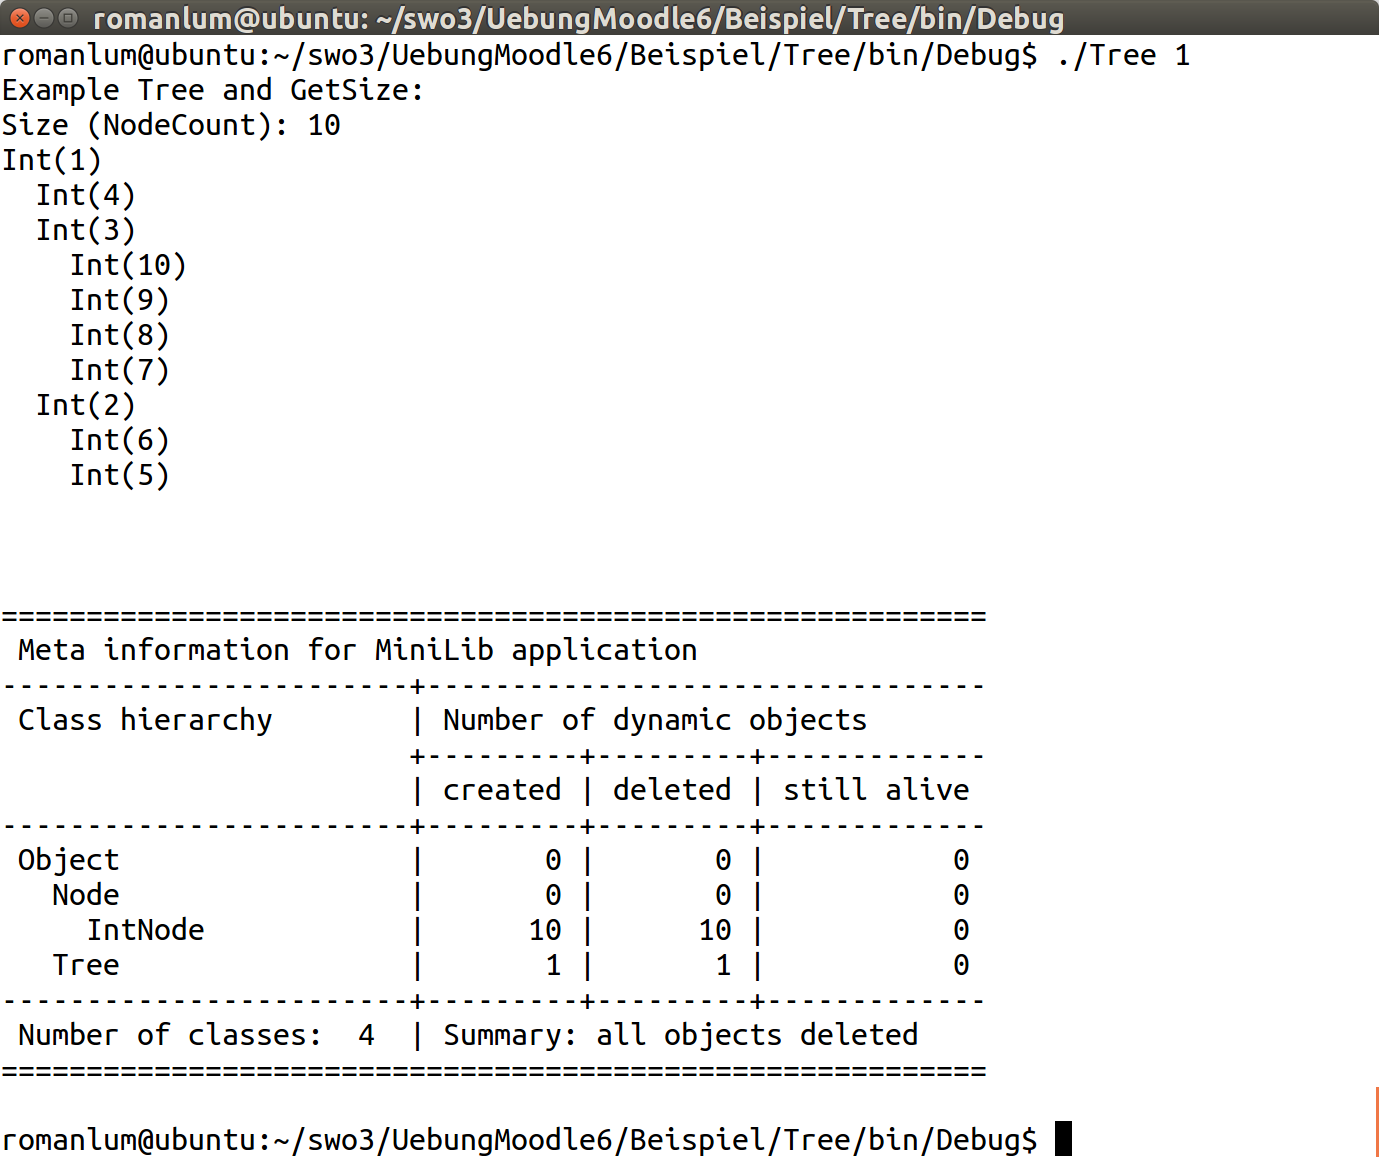
\includegraphics[width=400px, clip=true,trim=0px 000px 0px 0px]{../Screenshots/1.png}
\subsubsection{Testfall 2 - Methode DeleteSubtree}
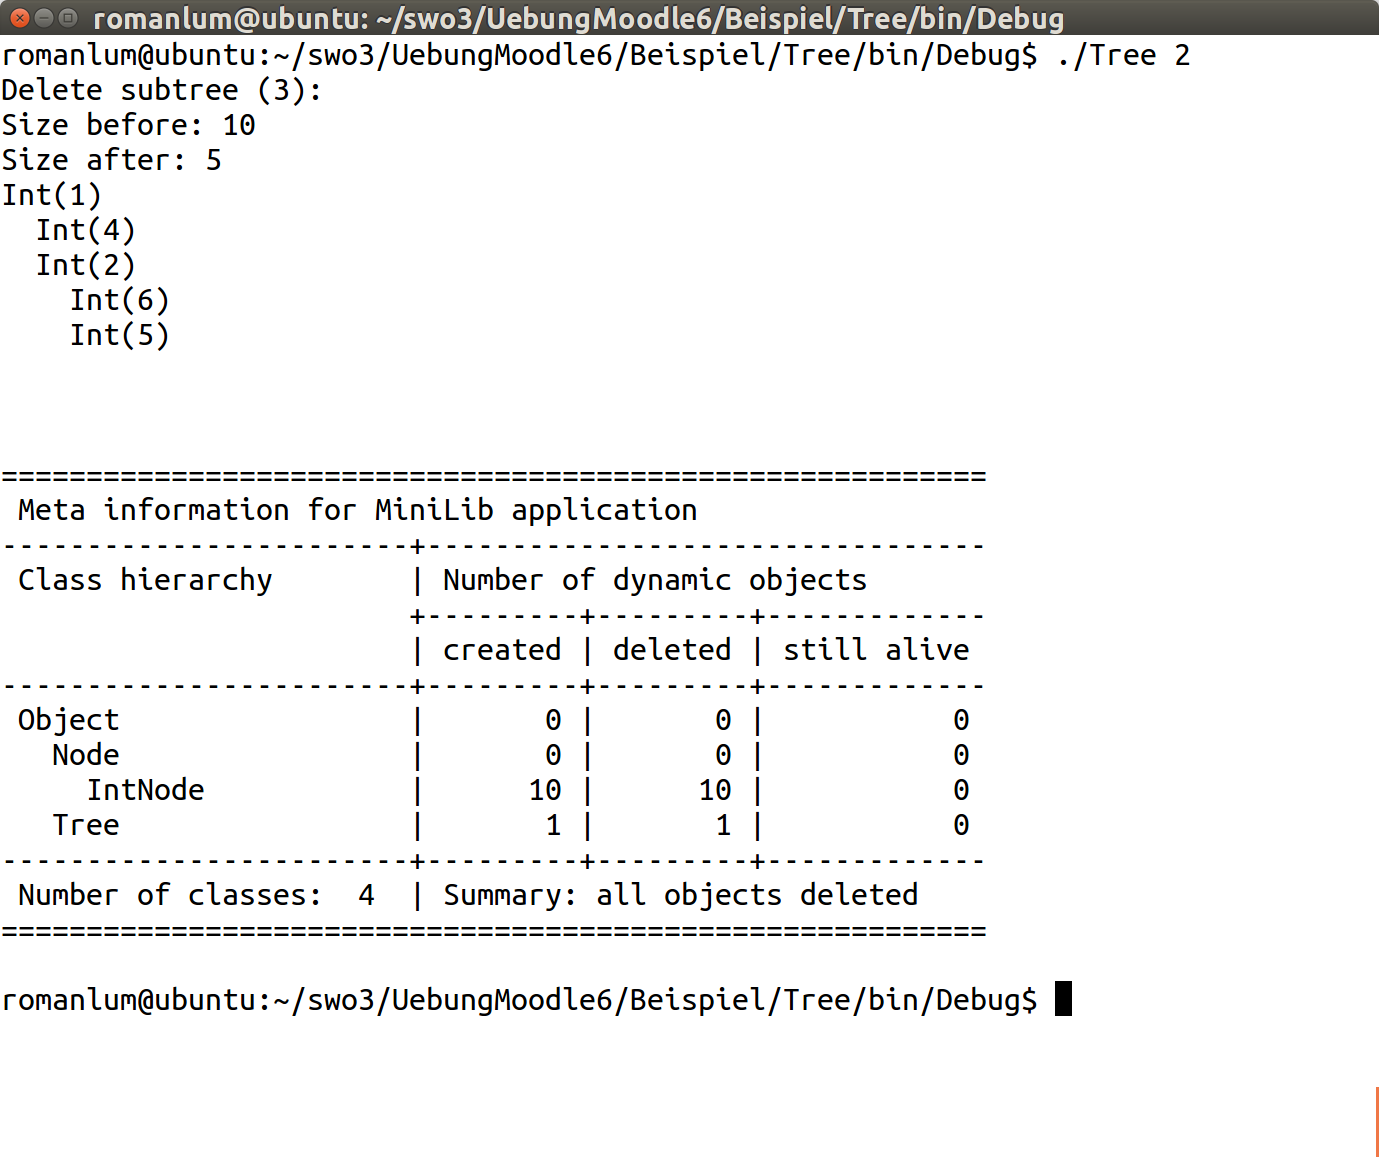
\includegraphics[width=400px, clip=true,trim=0px 200px 0px 0px]{../Screenshots/2.png}
\subsubsection{Testfall 3 - Methode DeleteElements}
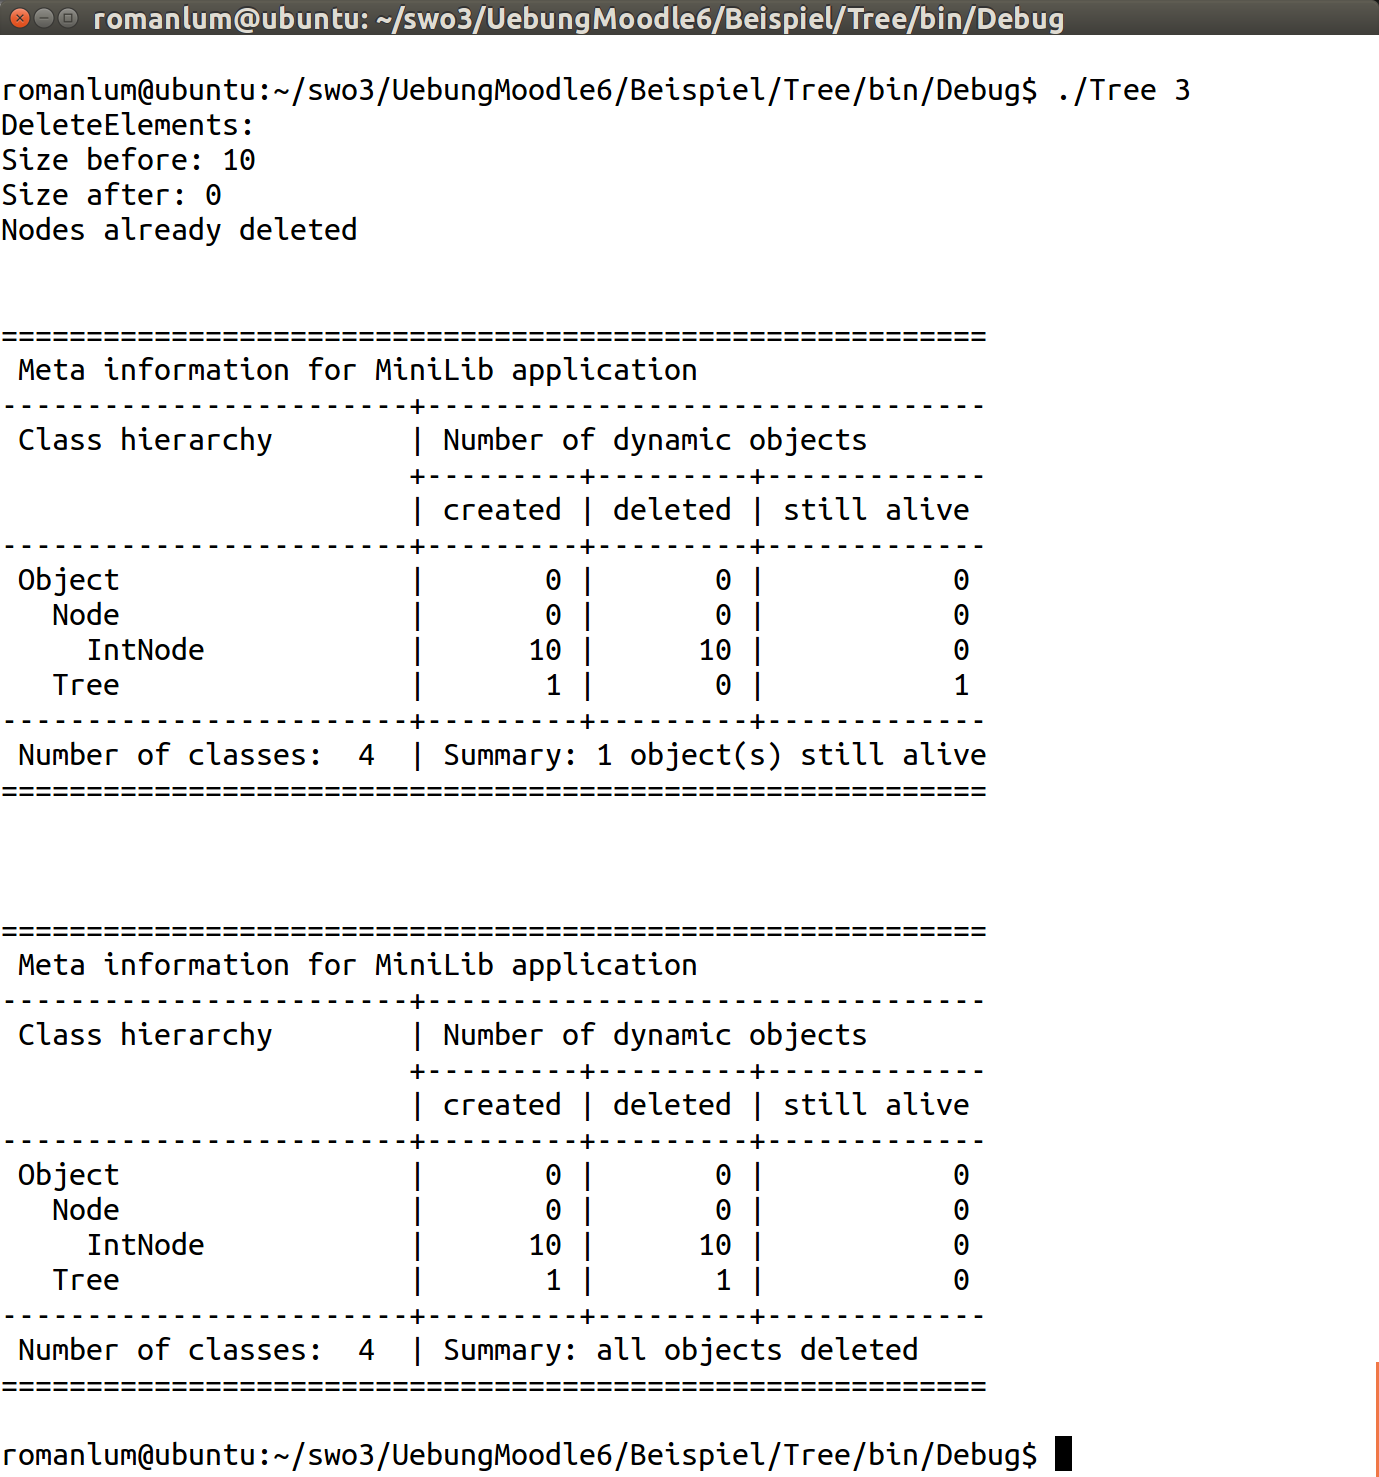
\includegraphics[width=400px, clip=true,trim=0px 000px 0px 0px]{../Screenshots/3.png}
\subsubsection{Testfall 4 - Methode Clear}

\includegraphics[width=400px, clip=true,trim=0px 000px 0px 0px]{../Screenshots/4.png}
\subsubsection{Testfall 5 - Tree - ung�ltige Operationen}
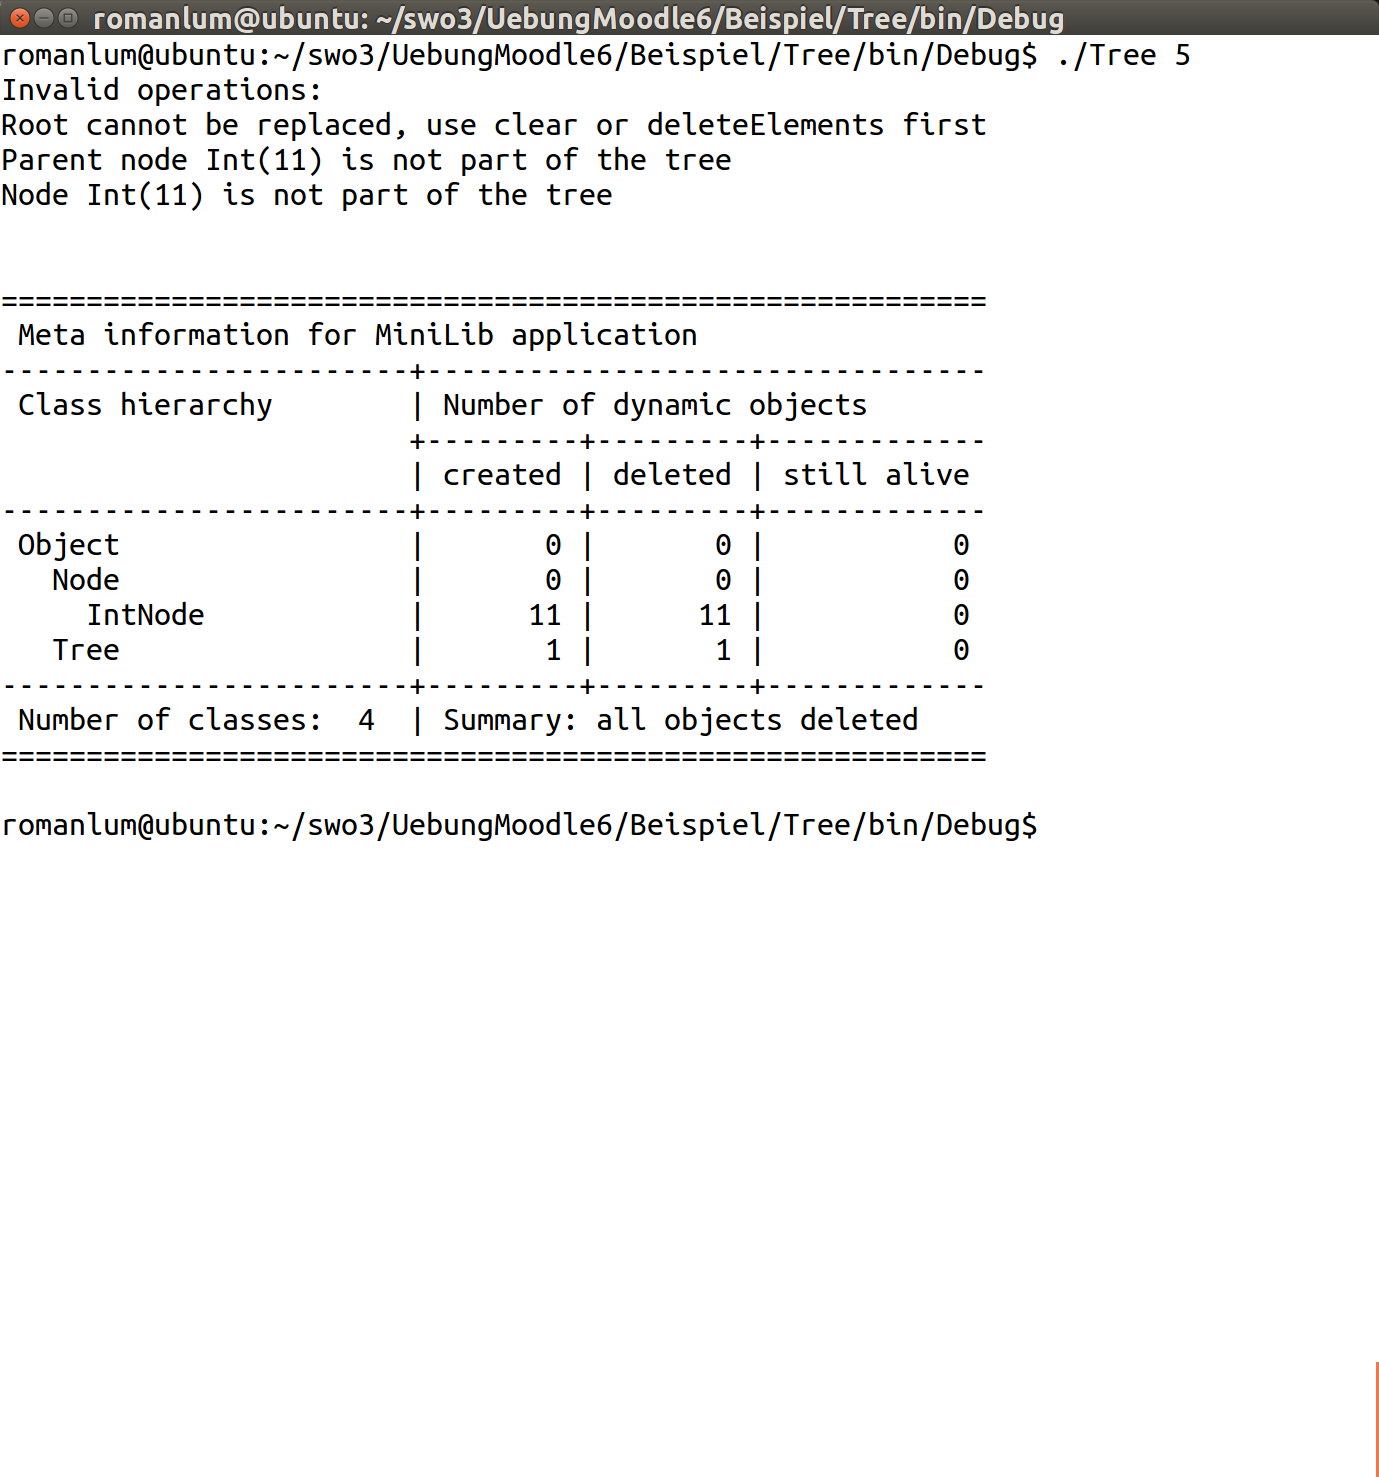
\includegraphics[width=400px, clip=true,trim=0px 200px 0px 0px]{../Screenshots/5.png}
\subsubsection{Testfall 6 - Tree - Kopierkonstruktor und Zuweisungsoperator}
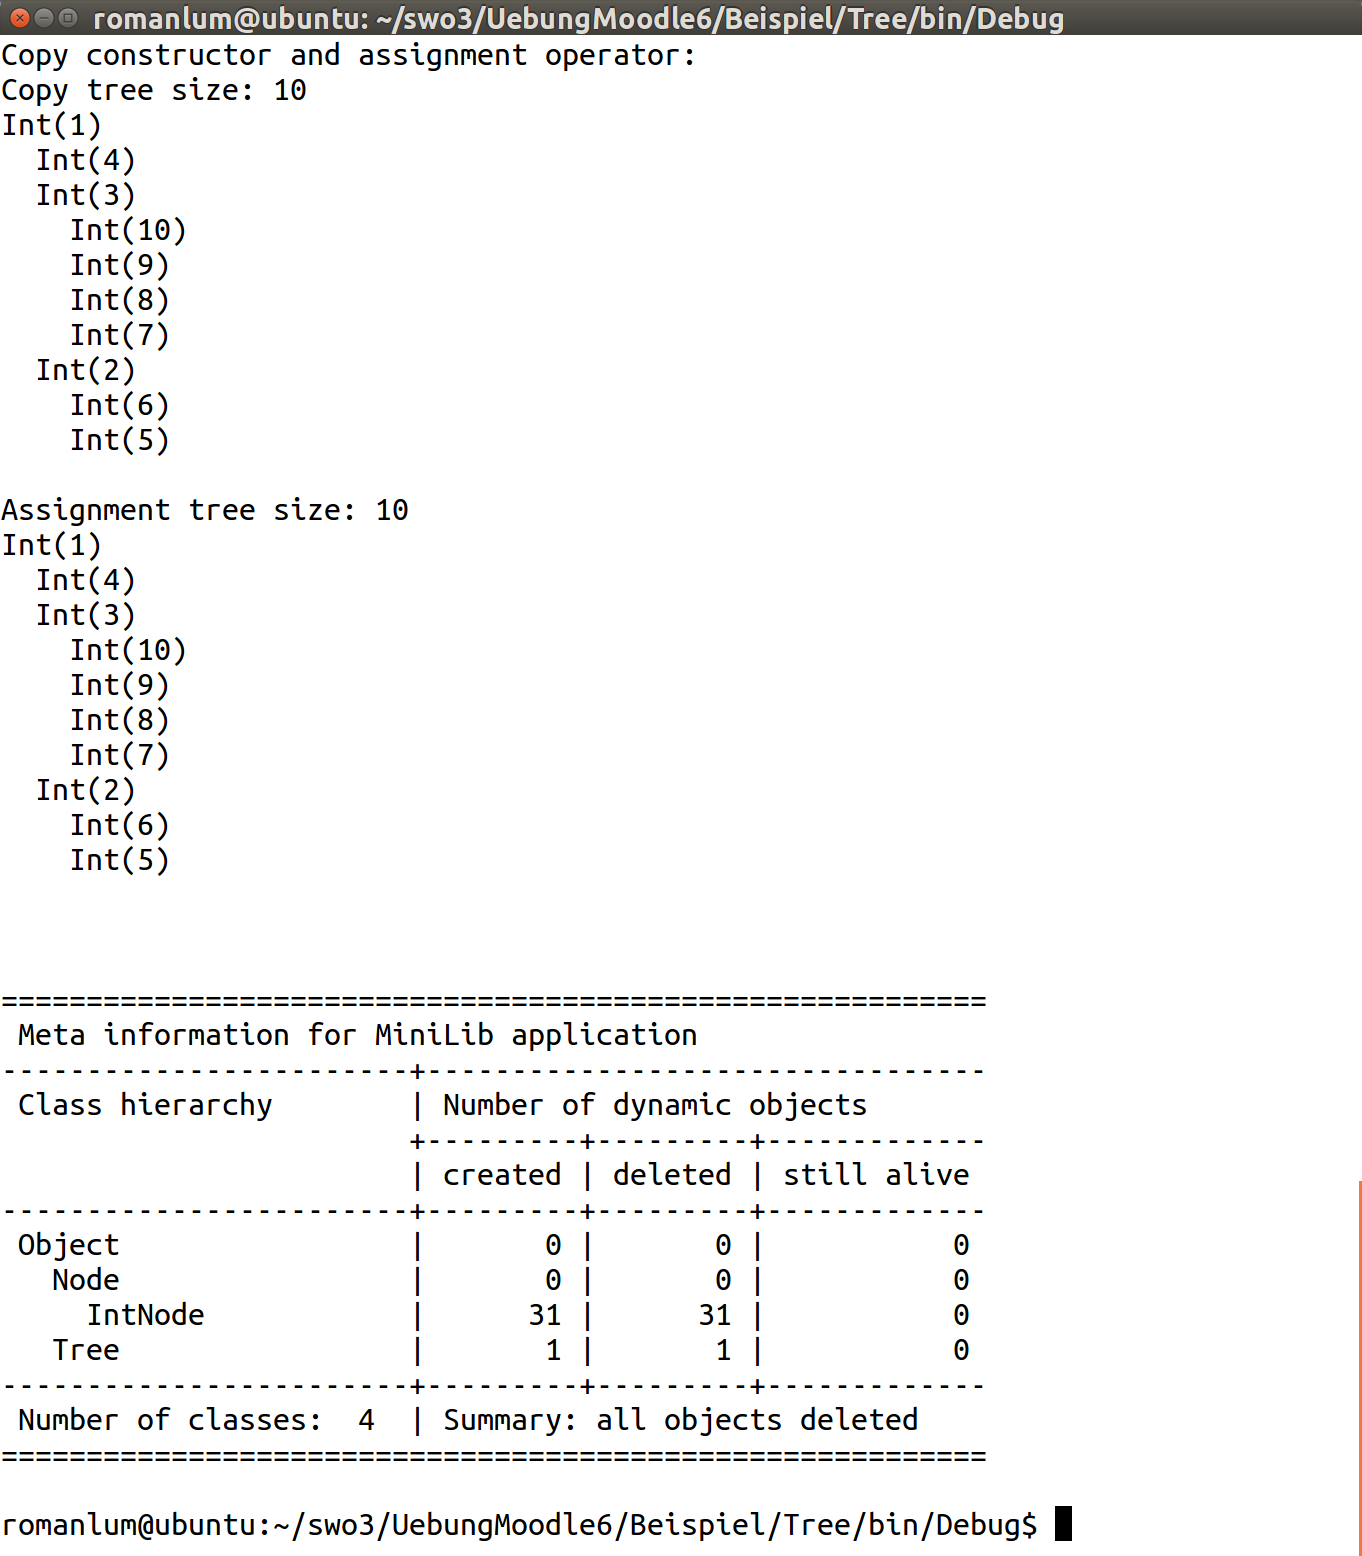
\includegraphics[width=400px, clip=true,trim=0px 000px 0px 0px]{../Screenshots/6.png}
\subsubsection{Testfall 7 - Dateisystem}
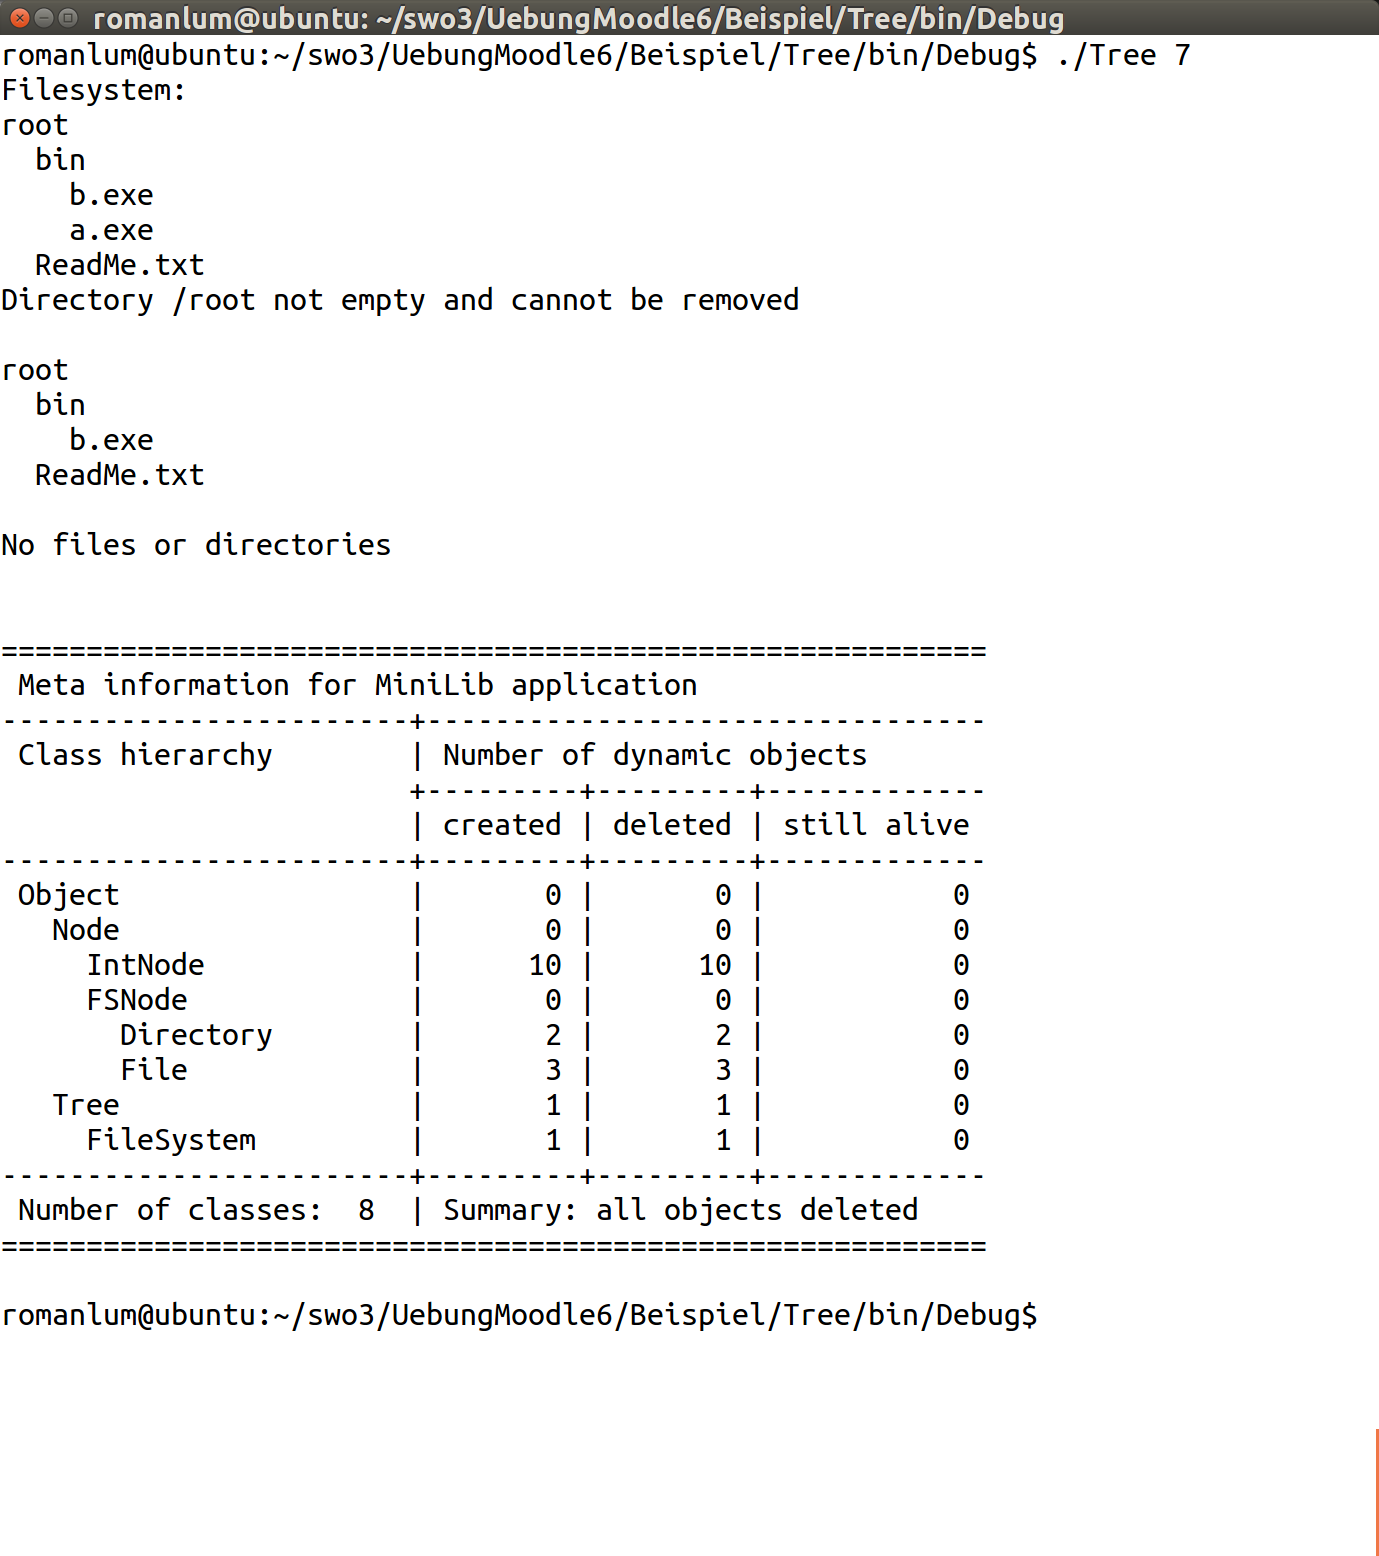
\includegraphics[width=400px, clip=true,trim=0px 200px 0px 0px]{../Screenshots/7.png}
\subsubsection{Testfall 8 - Dateisystem - ung�ltige Operationen}
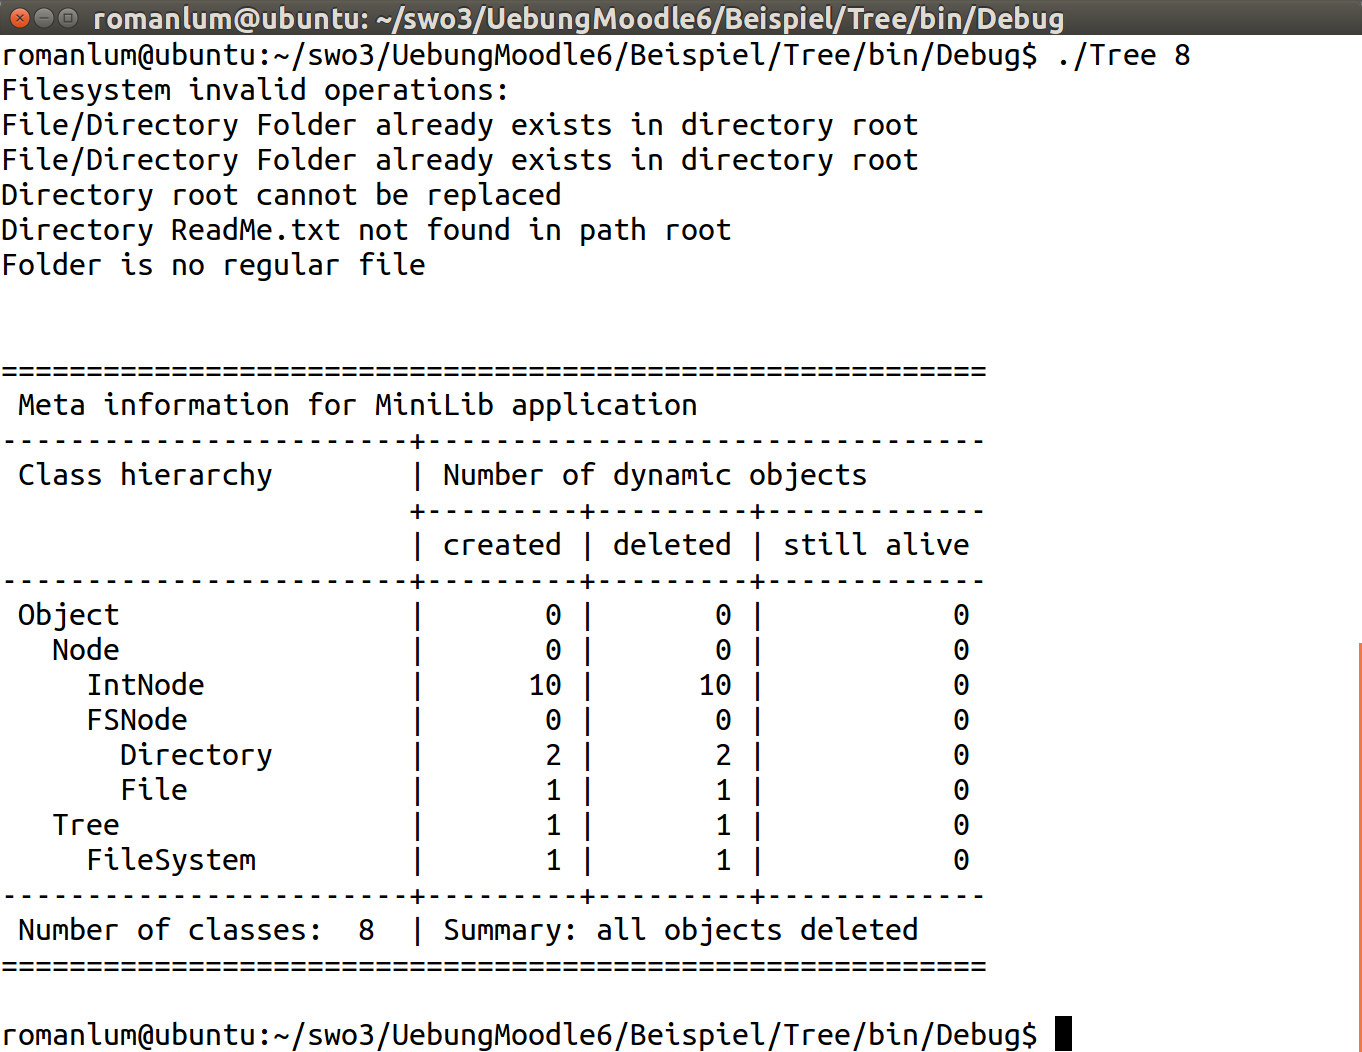
\includegraphics[width=400px, clip=true,trim=0px 100px 0px 0px]{../Screenshots/8.png}	

\end{document}